% resume.tex
% vim:set ft=tex spell:

\documentclass[10pt,a4paper]{article}
\usepackage[a4paper,margin=0.70in]{geometry}
\usepackage{graphicx}
\usepackage[utf8]{inputenc}
\usepackage[spanish]{babel}
\usepackage{mdwlist}
\usepackage{textcomp}
\usepackage{tgpagella}
\pagestyle{empty}
\setlength{\tabcolsep}{0em}

% indentsection style, used for sections that aren't already in lists
% that need indentation to the level of all text in the document
\newenvironment{indentsection}[1]%
{\begin{list}{}%
	{\setlength{\leftmargin}{#1}}%
	\item[]%
}
{\end{list}}

% opposite of above; bump a section back toward the left margin
\newenvironment{unindentsection}[1]%
{\begin{list}{}%
	{\setlength{\leftmargin}{-0.5#1}}%
	\item[]%
}
{\end{list}}

% format two pieces of text, one left aligned and one right aligned
\newcommand{\headerrow}[2]
{\begin{tabular*}{\linewidth}{l@{\extracolsep{\fill}}r}
	#1 &
	#2 \\
\end{tabular*}}

% and the actual content starts here
\begin{document}

\begin{center}
{\LARGE \textbf{Mario Daniel Ruiz Saavedra}}

Carrera 26 \# 10 - 13\ \ 
\ \ Urbanización Country Club Villas\ \ \textbullet
\ \ Puerto Colombia, Atlántico, Colombia
\\
310 626 1218\ \ \textbullet
\ \ desiderantes93@gmail.com\ \ \textbullet \ \ https://github.com/desiderantes
\\
CC. 1082976380 \ \ \textbullet \ \ Born in Barranquilla, \ \ 1993-08-04


\vspace{0.4em}
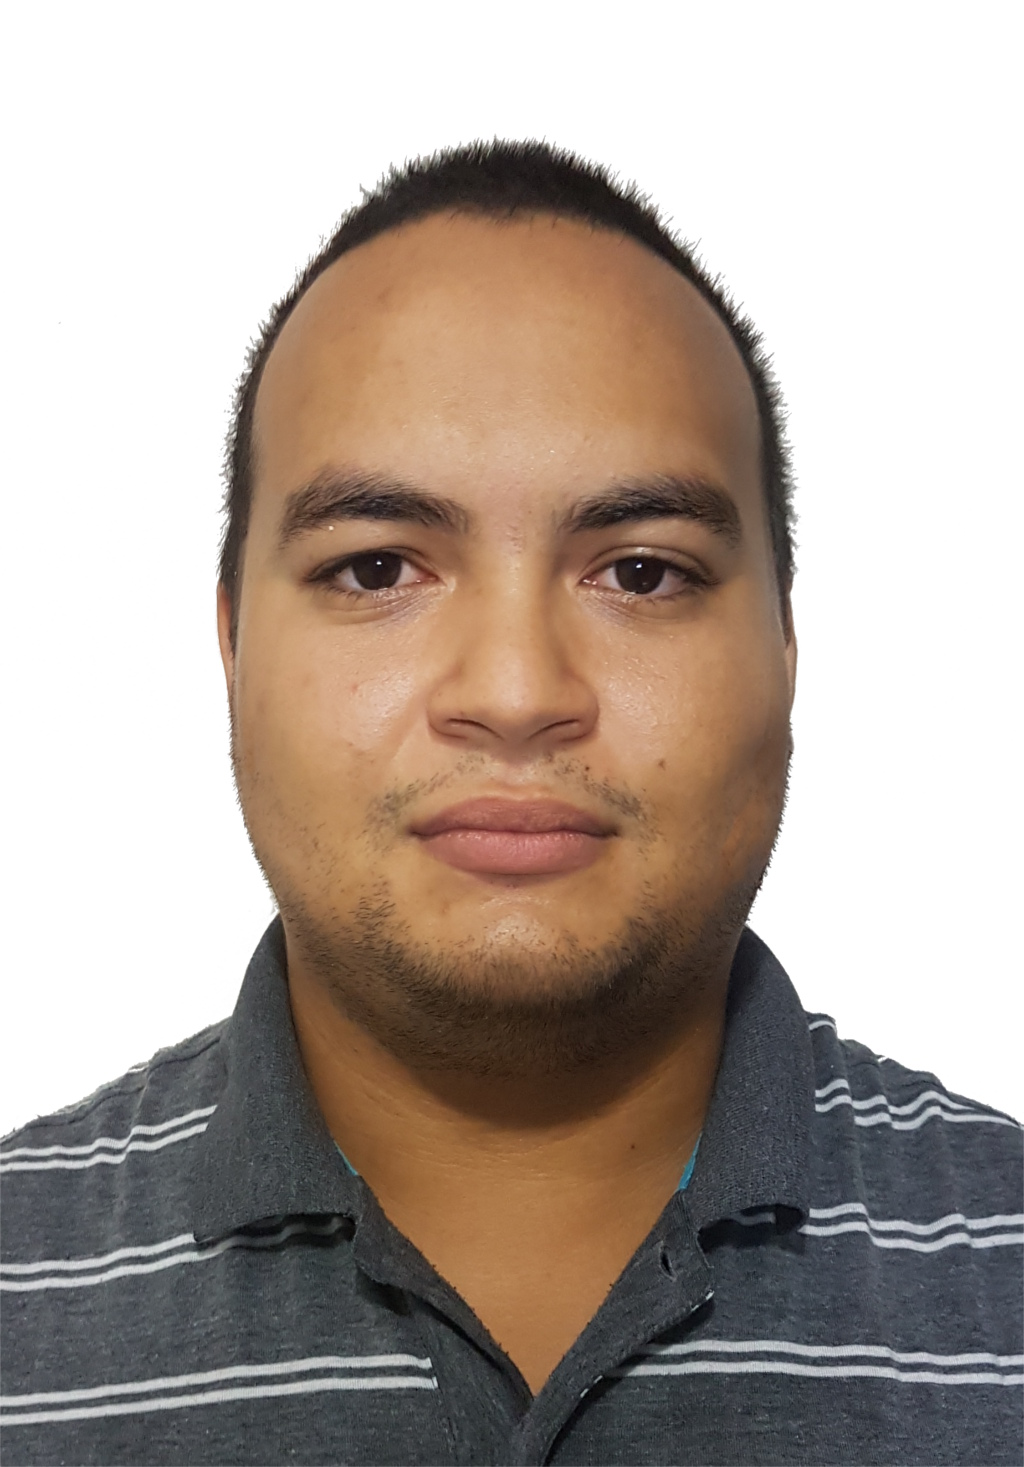
\includegraphics [width=6cm,height=6cm,keepaspectratio]{Foto.jpg}
\end{center}
\hrule
\vspace{-0.4em}
\subsection*{Experience}

\begin{itemize}
	\parskip=0.1em

	\item
	\headerrow
		{\textbf{Accendo S.A.S}}
		{\textbf{www.accendo.com.co}}
	\\
	\headerrow
		{\emph{Junior Developer}}
		{\emph{july 2015 - september 2016}}
	\begin{itemize*}
		\item 
		\headerrow
		{\textbf{TerraInnova}}
		{\emph{july 2015 – october 2015}}

		TerraInnova is an e-commerce and contact portal, specialized in agricultural commodities and keeping producers and consumers in touch. The development included a backend written in Java, using Spring MVC, jOOQ, PostgreSQL, and a frontend with Thymeleaf, Bootstrap and jQuery. The portal runs on CentOS 7, with AWS for the user data layer.
		
		\item 
		\headerrow
		{\textbf{WColombia}}
		{\emph{october 2015 – march 2016}}
		A web tool for inventory management and income/expense tracking of slot machines, taking into account taxes and goverment regulations. I worked  on the backend side, with Java 8,  Spring Framework MVC, JPA, Hibernate, jOOQ and PostgreSQL.
		\item 
		\headerrow
		{\textbf{Crisálida}}
		{\emph{january 2016 – april 2016}}
		Crisálida is a government program to educate about  sexual relationships, coexistence and child’s rights. Our portal managed surveys, student inscriptions, situational alarms, and report bulding (as a .xls file). The
		backend uses Spring Data, Spring MVC, Spring Boot, jOOQ, and PostgreSQL. Frontend-wise, it uses Javascript (JSX) with React, Redux in the data layer, and a Bootstrap 3- based design.
		\item 
		\headerrow
		{\textbf{Sushi2Home}}
		{\emph{may 2016 – july 2016}}
		Sushi2Home is a sushi delivery service, available vía social media and its own website. It consists of a server in Ruby-on-Rails, with PostgreSQL and a customized instance of an e-comerce platform, Shoppe. I worked mainly on the consumer-facing frontend, where I helped with the auto-combo generation, and a C{$^\sharp$} (WPF) desktop client to handle incoming orders, aurtomatic receipt printing, and delivery assignment.
		\item 
		\headerrow
		{\textbf{Trackvy}}
		{\emph{december 2015 – september 2016}}
		Trackvy is a RFID-based stock management system. I worked on a port of the C{$^\sharp$} Windows CE Reader client to a new API version; a new readings portal for tool lending in C{$^\sharp$}, Windows Forms, and SQLite; a new version of the tagging and movement desktop tool in Java 8, JavaFX, H2, and Spring Context; and a port of the frontend from Angular 1 + Typescript+ D3.js to HTML5, jQuery, Chartist.js, Bootstrap and Thymeleaf. 
	\end{itemize*}

\end{itemize}

\begin{itemize}
	\parskip=0.1em
	
	\item
	\headerrow
	{\textbf{Nativapps S.A.S}}
	{\textbf{www.nativapps.com}}
	\\
	\headerrow
	{\emph{Java Developer}}
	{\emph{february 2017 -}}
	\begin{itemize*}
		\item 
		\headerrow
		{\textbf{OpenMDM}}
		{\emph{febuary 2017 –}}
		
		OpenMDM is a mobile device management platform. It can track a device’s location, battery info, and connection status. It also includes a remote management module vía web browser, and a command execution system. I’m currently writing the backend with Java 8, Spring Framework, jOOQ, ActiveMQ, and Swagger for the API documentation. I’m also currently involved in the remote acces client in Android, using a custom, stripped down VNC client written in Java.
		\end{itemize*}
	
\end{itemize}

\hrule
\vspace{-0.4em}
\subsection*{Certifications}

\begin{itemize}
	\parskip=0.1em

	\item 
	\headerrow
		{\textbf{Programación de páginas Web con HTML y JavaScript}}
		{\textbf{SENA}}
	\\
	\headerrow
		{\emph{Licencia SGCV20102985332}}
		{\emph{diciembre de 2010}}
	\begin{itemize*}
		\item Web dev with HTML, ECMAScript 5 \& CSS 3
	\end{itemize*}

\end{itemize}

\hrule
\vspace{-0.4em}
\subsection*{Educación}

\begin{itemize}
	\parskip=0.1em

	\item 
	\headerrow
		{\textbf{Colegio Gimnasio Bolivariano}}
		{\textbf{Santa Marta, Colombia}}
	\\
	\headerrow
		{\emph{HS grad with emphasis in natural science}}
		{\emph{1997 - 2009}}

	\item 
	\headerrow
	{\textbf{Universidad del Norte}}
	{\textbf{Barranquilla, Colombia}}
	\\
	\headerrow
	{\emph{Systems and Computing Engineering}}
	{\emph{2012 - (en pausa)}}
	\begin{itemize*}
		\item I want to focus on system programming in ether a UNIX-like system or a UNIX-next system (like Plan 9)
		\item Writing useful subsystems in a message-passing platform is the way to go.
	\end{itemize*}
	
\end{itemize}


\hrule
\vspace{-0.4em}
\subsection*{Trade skills}

\begin{indentsection}{\parindent}
\hyphenpenalty=1000
\begin{description*}
	\item[Programming (and not-so-programming) Languages:]
	C, Vala, Java, JavaScript, \LaTeX, HTML, C{$^\sharp$}, JSX, SQL
	\item[Frameworks \& Libraries:]
	Spring (Boot, MVC, Data, Cloud, JPA), React, Redux, jQuery, Bootstrap 3, Hibernate, Thymeleaf, jOOQ, JavaFX, Glade, WPF.
	\item[Tools:]
	GNU/Linux, Git, Vagrant, IntelliJ IDEA, nano, KVM, GIMP, Inkscape, LibreOffice Writer
	\item[Free software contributions:]
	ValaVerbalExpressions (author), SDL2 Bindngs for Vala (coauthor), Stew build system (maintainer)
\end{description*}
\end{indentsection}
\hrule
\vspace{-0.4em}
\subsection*{Referrals}
\begin{indentsection}{\parindent}
\hyphenpenalty=1000
\begin{description*}
	\item[Family:]
	
	\begin{itemize*}
		\
		\item
		\item Carmen Nidia Saavedra Ruz - Lawyer - 3103631187
		\item Hernan Darío Ruiz Soler - Systems Engineer - 3013437656
		\item Ruben Darío Ruiz Becerra - Mechanical Engineer - 3103574030
	\end{itemize*}

	\item[Personal:]
	
	\begin{itemize*}
		\
		\item
		\item Stefanny Espinosa - Electronic Engineer -  3145951482
		\item Carlos Arbey Bolaños Duarte - Electronic Engineer -  3005307422
		\item Jhon Jairo Ruiz Soler - Anthropologist - 3002426851
	\end{itemize*}
\end{description*}
\end{indentsection}

\end{document}
